
\pgfmathsetmacro{\gridWidthCm}{\textwidth/1cm}
\newdimen\tikzspacer
\tikzspacer=18pt

\rpt[10]{
\section{dots}
\newdimen\spaceleft
\spaceleft=\dimexpr\textheight-\pagetotal-\tikzspacer\relax
\pgfmathsetmacro{\gridHeightCm}{\spaceleft/1cm}
% Needed to subtract an extra 14pt to prevent the page content from jumping
% to the next page in some cases.
  \begin{tikzpicture}
    \foreach \x in {0,0.5,...,\gridWidthCm}
    \foreach \y in {0,0.5,...,\gridHeightCm}
    {
  \fill (\x cm,\y cm) circle (0.015cm);
    }       
  \end{tikzpicture}
  \pagebreak
}
\rpt[10]{
  \section{triangular}
  \newdimen\spaceleft
  \spaceleft=\dimexpr\textheight-\pagetotal-\tikzspacer\relax
  \pgfmathsetmacro{\gridHeightCm}{\spaceleft/1cm}
  \begin{tikzpicture}
    \foreach \x [count=\xi] in {0,0.5,...,\gridWidthCm}
    \foreach \y [count=\yi] in {0,1,...,\gridHeightCm}
    {
  \fill (\x cm,\y cm) circle (0.015cm);
    }       
    \foreach \x [count=\xi] in {0.25,0.75,...,\gridWidthCm}
    \foreach \y [count=\yi] in {0.5,1.5,...,\gridHeightCm}
    {
  \fill (\x cm,\y cm) circle (0.015cm);
    }       
  \end{tikzpicture}
  \pagebreak
}
\rpt[6]{
 \section{graph}
  \newdimen\spaceleft
  \spaceleft=\dimexpr\textheight-\pagetotal-\tikzspacer\relax
  \pgfmathsetlengthmacro{\graphWidth}{\textwidth - mod(\textwidth,0.5cm)}
  \pgfmathsetlengthmacro{\graphHeight}{\spaceleft - mod(\spaceleft,0.5cm)}
  % Have to use mod here to get an even number of grid cells
  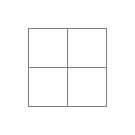
\begin{tikzpicture}
\draw [very thin, gray, step=0.5cm] (0,0) grid (\graphWidth,\graphHeight);
  \end{tikzpicture}
\pagebreak
}
\rpt[10]{
 \section{blank}
\pagebreak
}

